
\section{Learning object appearance}

The affordance learning in the last section depended on a mechanism
for differentiating objects based on their color histogram.
%The data collected over hundreds of pokes contained a significant...
%
By clustering segmented views of objects in this way,
the robot collected about 100 views of each object.  
If the quality of the clusters generated is sufficiently good, it
should be possible to extract reliable consensus prototypes for each 
object.  This is in fact the case, as Figure~\ref{fig:auto-proto}
shows.  Using the most naive alignment procedure and averaging
process possible, a blurry ``mean'' view of the objects can
quickly be derived.  This could be sharpened by better alignment
procedures, or just used to pick out the best single match
to the mean view for each object.
%
Of course, this paper is not proposing that simple color histograms
are how recognition should be done~-- there are better ways (for
example, see~\cite{schiele00recognition}), rather it is giving
evidence that shared activity can generate data of sufficient quality
to train up detailed, accurate models of objects in the robot's 
environment.

%
\begin{figure}[tb]
\begin{center}
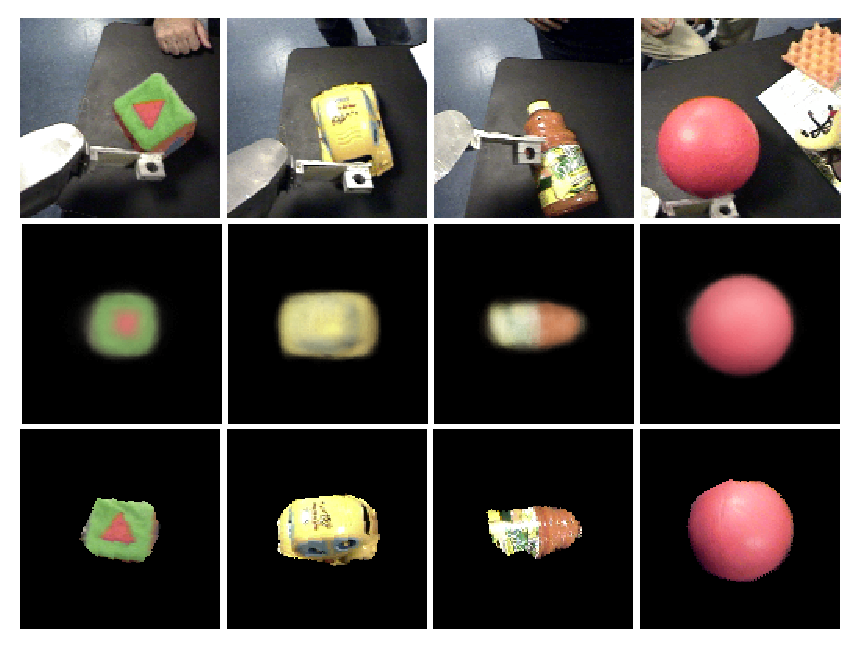
\includegraphics[width=\columnwidth]{fig-auto-proto.eps}
\caption{ 
\label{fig:auto-proto}
%
The top row shows the four objects used in this 
experiment, seen from the robot's perspective.  The 
middle row shows prototypes derived for those objects
using a na\"{\i}ve alignment procedure.  
%All the views
%of a single object (as determined by color histogram
%comparison) were aligned horizontally based on
%their segmentations.  The views were then simply 
%averaged, along with their masks, producing the
%result shown here.  
None of the prototypes contain
any part of the robot's manipulator, or the 
environment.  These prototypes are used 
to find the best available segmentations
of the objects (bottom row).
%
}
\end{center}
\end{figure}


